\section{Unit testing}
Unit testing is our primary way of testing our system, and belongs in the dynamic white-box testing category.
The purpose of unit testing is to see if an isolated subset of the system works as expected, given some pre-defined input \cite{TestDrivenDevelopment}.
For this project, unit tests are utilized for both the React frontend and the API, to ensure that the system works as intended.

\subsection{Choice of framework}
One of the first decisions when creating unit tests, is the choice of test runner.
Since the React library is shipped with Jest \cite{ReactRunningTests}, and since both parts of the system are JavaScript based, it seemed like the optimal solution to use the same test runner.
However, after using Jest for testing the API for a while, several issues surfaced when trying to implement mock functions related to our ORM and some TypeScript functionality in general.
These problems were related to the type security provided by TypeScript that TypeORM utilizies, meaning that TypeORM had a security feature where it would ensure that it was only called with real objects and not stubs created by Jest.
To simplify the creation of unit testing on the API, the test driver for this was changed to Mocha, since it uses another approach to creating stub objects, which worked out of the box.

One of the main differences between Jest and Mocha is that Jest is a complete suite that supports running the tests, asserting results, stubbing, test coverage and much more.
Mocha, on the other hand, is just a test runner and requires additional libraries for asserting, stubbing and generating code coverage results \cite{Mocha}.
We chose to use Chai for assertions, Sinon for stubbing and Nyc for generating code coverage.

\subsection{What to test}
The answer to what should be tested varies a lot between the frontend and the API.
One of the axioms of testing states that it is impossible to test a program completely, and should be seen as a risk-based exercise where the tester asserts which parts of the system should be tested, and how thoroughly it should be tested \cite{SoftwareTesting}.
For the frontend of the system, it would be possible to test whether each component is rendered to the user, if all the information is correct, what happens if you use 0 as input to the function, 1 as input, 3 as input.. And so on.
Instead, we chose to focus on testing if the components that are conditionally rendered are shown when the conditions are fulfilled.
An example of this could be the \textit{Show User} page, where the system should show tutor info if and only if the user is actually a tutor.
This now leads to test cases like is the info rendered if:
\begin{itemize}
    \item the user is a tutor?
    \item the user is a tutor, but the tutor information is invalid?
    \item the user is a tutor, but the tutor information is incomplete?
\end{itemize}

In addition to the conditional rendering, any business logic located on the frontend should be tested to ensure both that it works as intended, but also that any future updates to the code will not break it, which is referred to as regression testing.
This security is done by enforcing that all unit tests must run before the feature can be merged into the development branch of the system.

For the API, some functionality like the ORM is handled by external packages.
Since this is not code we are writing ourselves, we have chosen to assume that the developers of the packages have tested the software and thus we will not have to.
We focus on unit testing our controllers and middleware to ensure that they work as expected, and instead do some integration testing for the external packages, to ensure that they work as expected when integrated into our system.
This will be further described in \autoref{sec:integrationTesting}.

\subsection{Stubbing}
A major obstacle for generating our tests was to avoid the calls to the ORM in the API, which would connect to the database.
At first, we considered different ways to handle this connection, such as having a test database that would be wiped before each test to generate a controlled environment.
However, after doing more research we realized that instead of connecting to a real world configuration, it would be beneficial to be able to control exactly which values should be returned.
This principle is called stubbing \cite{SoftwareTesting}.
The idea is that instead of calling a given function, we create a stub function that is called instead.
An example of this can be seen in the unit test in \autoref{lst:unitTestStubbing}, where we stub the function call to \texttt{getByEmail} in the \texttt{userService}.
In the real code, the code seen on \autoref{lst:getByEmail} would be called as a part of the call to the login function on line 16, which connects to the database, but instead of doing so we use the Sinon library to stub the function, and tell it to throw an exception instead, so we can see how the controller handles this case.

\begin{lstlisting}[caption={Unit test with stubbing},label={lst:unitTestStubbing}]
...
it('returns status 400 if service throws exception', async function() {
    const request = {
        body: {},
    };
    const req = mockReq(request);

    const res = mockRes({
        status: function(s: number) {
            this.statusCode = s;
            return this;
        },
    });
    const stubResult = sinon.stub(userService, 'getByEmail').throws('exception');

    await AuthController.login(req, res);
    expect(res.statusCode).to.equal(400);
    stubResult.restore();
});
...
\end{lstlisting}

\begin{lstlisting}[caption={Actual getByEmail function},label={lst:getByEmail}]
static getByEmail = async (email: string): Promise<User> => {
    //Get user from database
    const userRepository: Repository<User> = getRepository(User);
    return await userRepository.findOneOrFail({ where: { email } });
};
\end{lstlisting}

As seen on \autoref{lst:unitTestStubbing} lines 3 to 13, we also made use of mocking for defining the request and response parameters used for requests to the controller.
This allows us to check whether the correct status code is returned from the controller by overriding the status function.
Normally, the function would set the headers that are returned to the client requesting the API.
However, for this test we are only interested in seeing which parameter the status function is called with to ensure that it matches our expectations.
This way it is now possible to check if the \texttt{statusCode} property on the response is set to what we expect, as seen on line 17.

Finally, the stub is restored to make sure that it only behaves in this limited way in the scope of the unit test.

\subsection{Metrics of good testing}
There are multiple ways of measuring whether the created unit tests are sufficient.
Our primary metric for our automated tests are code coverage, which measures how much of the code base is covered by unit tests.
This is split into four categories: statement coverage, branch coverage, function coverage and line coverage.

\begin{figure}[H]
    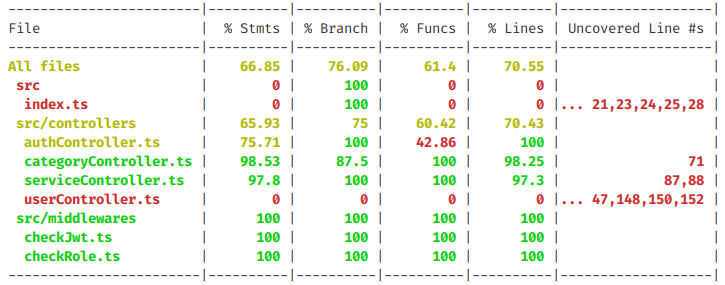
\includegraphics[width=\linewidth]{/test.png}
     \caption{The output of the code coverage reporter NYC}
     \label{fig:testResults}
 \end{figure}

We used a configuration to report files with 0-50\% coverage as red, 50-75\% as yellow and 75-100\% as green.
While this is a good indicator of how much of the code has been tested, it does not ensure that the tests are useful and correct.

To ensure this, we make use of formal reviews of all changes made to the code and tests.
